\documentclass[letterpaper,11pt,nointlimits,reqno]{amsart}
\pagestyle{headings}

% Packages
\usepackage{accents}
\usepackage{array}
\usepackage{booktabs}
\usepackage{enumerate}
\usepackage{fancyhdr}
\usepackage[final]{graphicx}
\usepackage{fullpage}
\usepackage{lastpage}
\usepackage{listings}
\usepackage{longtable}
\usepackage{mathrsfs}
\usepackage{mathtools}
\usepackage[numbers,sort&compress]{natbib}
\usepackage[usenames,dvipsnames,svgnames,table]{xcolor}

% Avoids xcolor options clashes
\usepackage{pgfplotstable}

% In conjunction with -shell-escape, automatically convert EPS to PDF
\usepackage{epstopdf}
\epstopdfsetup{outdir=./,suffix=-generated,update,verbose}
\epstopdfDeclareGraphicsRule{.eps}{pdf}{.pdf}{%
    epstopdf --outfile=\OutputFile \space `kpsewhich \space "\SourceFile"`
}

% Hyperref package must be last otherwise the contents are jumbled
% hypertexnames disabled to fix links pointing to incorrect locations
\usepackage[hypertexnames=false,final]{hyperref}

\mathtoolsset{showonlyrefs,showmanualtags}
% \allowdisplaybreaks[1] % Allow grouped equations to be split across pages

% Document-specific commands
\newcommand{\Mach}[1][]{\mbox{Ma}_{#1}}

% From how-to-prevent-a-page-break-before-an-itemize-list
% http://tex.stackexchange.com/questions/2644
\makeatletter
\newcommand\mynobreakpar{\par\nobreak\@afterheading}
\makeatother

% Configure inline code listings
\lstset{
  basicstyle=\footnotesize\sffamily,
  columns=fixed,
  commentstyle=\color{blue},
  firstnumber=1,
  frame=single,
  keepspaces=true,
  numberfirstline=true,
  numbersep=7pt,
  numbers=left,
  numberstyle=\tiny\color{darkgray},
  showstringspaces=false,
  showtabs=false,
  stepnumber=5
}

\begin{document}

\title{Favorable pressure gradient base flow computations}
\author{Rhys Ulerich}

\begin{abstract}
This document discusses how to obtain a favorable pressure gradient base flow
for use within temporally homogenized boundary layer simulations.  First, a
compressible potential flow problem is formulated for a radially symmetric
source or sink flow.  This one-dimensional problem is cast into a form
commodity ODE integrators can solve to obtain primitive state as a function of
radius.  The solution is then mapped from $\left(r,\theta\right)$ into
$\left(x,y\right)$ coordinates and a base flow profile extracted from some constant
$x$ line segment.  The segment chosen, as well as the radial problem boundary
conditions used, are taken to match some boundary layer edge state of interest
using a numerical optimization procedure.  Finally, this procedure is used
to produce base flows in the spirit of laminar CEV heat shield conditions.
\end{abstract}

\maketitle

\tableofcontents

%%%%%%%%%%%%%%%%%%%%%%%%%%%%%%%%%%%%%%%%%%%%%%%%%%%%%%%%%%%%%%%%%%%%%%%%%%%%%%%%
\section{The nondimensional, compressible potential flow equation}
%%%%%%%%%%%%%%%%%%%%%%%%%%%%%%%%%%%%%%%%%%%%%%%%%%%%%%%%%%%%%%%%%%%%%%%%%%%%%%%%

A particularly crisp derivation of the coordinate-independent,
velocity-potential formulation of the compressible potential flow equations
appears in section II.A of \citet{Saad2011Coordinate}.  Their presentation
essentially is recounted here but velocity potential notation is suppressed.
Wherever necessary, sufficient smoothness is assumed.

The steady, inviscid momentum equation in an irrotational flow yields
\begin{align}
    \vec{\nabla}p
    &= -\rho \vec{u}\cdot\vec{\nabla}\vec{u}
     = -\rho \left(   \frac{1}{2}\vec{\nabla}\left(\vec{u}\cdot\vec{u}\right)
                    - \vec{u}\times\vec{\nabla}\times\vec{u}
        \right)
     = - \frac{1}{2} \rho \vec{\nabla}\vec{u}^2
\label{eq:momentum}
.
\end{align}
The irrotational velocity could be replaced by the gradient of a scalar
potential, \emph{viz.}
\begin{align}
  \vec{u} = \vec{\nabla}\phi + \vec{\nabla}\times\vec{A} = \vec{\nabla}{\phi}
  .
\end{align}
From the definition of the speed of sound~$a$, an isentropic assumption,
and equation~\eqref{eq:momentum},
\begin{align}
    \left(\frac{\partial p}{\partial \rho}\right)_{s} = a^2
    \implies
    \vec{\nabla}\rho = \frac{1}{a^2} \vec{\nabla} p
                     = - \frac{\rho}{2a^2} \vec{\nabla}\vec{u}^2
\label{eq:gradrho_gradp_relationship}
.
\end{align}
Expanding the steady continuity equation and
applying~\eqref{eq:gradrho_gradp_relationship},
\begin{align}
  0 &= \vec{\nabla}\cdot\rho\vec{u}
     = \rho\vec{\nabla}\cdot\vec{u} + \vec{u}\cdot\vec{\nabla}\rho
     = \rho\vec{\nabla}\cdot\vec{u}
     - \frac{\rho\vec{u}}{2a^2} \cdot \vec{\nabla}\vec{u}^2
\label{eq:continuity}
.
\end{align}
Because $\rho>0$ and $a>0$, for nontrivial $\vec{u}$ the above
equation may only be satisfied when
\begin{align}
       \frac{1}{2} \vec{u}\cdot \vec{\nabla}\vec{u}^2
    &= a^2 \vec{\nabla}\cdot\vec{u}
.
\label{eq:momentum_and_continuity}
\end{align}

Following \citeauthor{Saad2011Coordinate}, we invoke that stagnation energy
stays constant throughout such a flow to connect the local speed of sound to
reference parameters and the local velocity.  That is, for flow enthalpy $h =
a^2 / \left(\gamma-1\right)$, reference enthalpy $h_0 = a_0^2 /
\left(\gamma_0-1\right)$, and reference velocity $u_0$,
\begin{align}
        \frac{a^2  }{\gamma  -1} + \frac{1}{2} \vec{u}^2
     &= \frac{a_0^2}{\gamma_0-1} + \frac{1}{2} u_0^2
\end{align}
holds everywhere.  Notice the ideal gas equation of state, $\rho a^2 = \gamma
p$, was not imposed and it therefore will not be satisfied in general.  After a
small rearrangement, our energy constraint
\begin{align}
        a^2
     &=   \frac{\gamma-1}{\gamma_0-1} a_0^2
        + \frac{\gamma-1}{2} \left(u_0^2 - \vec{u}^2\right)
\label{eq:stagnation_sound}
\end{align}
may be used within equation \eqref{eq:momentum_and_continuity} to obtain
\begin{align}
       \vec{u}\cdot \vec{\nabla}\vec{u}^2
    &= \left[
          2 \frac{\gamma-1}{\gamma_0-1} a_0^2
        + \left(\gamma-1\right) \left(u_0^2 - \vec{u}^2\right)
       \right]\vec{\nabla}\cdot\vec{u}
.
\end{align}
Adding a constant $\gamma=\gamma_0$ assumption, one finds the dimensional result
\begin{align}
       \vec{u}\cdot \vec{\nabla}\vec{u}^2
    &= \left[
          2 a_0^2
        + \left(\gamma_0-1\right) \left(u_0^2 - \vec{u}^2\right)
       \right]\vec{\nabla}\cdot\vec{u}
\label{eq:cpfgibbs_dim}
.
\end{align}

To nondimensionalize, chose some reference length $l_0$ and declare
\begin{align}
    x     &= x^\ast l_0
&   a     &= a^\ast a_0
&   u     &= u^\ast u_0 = u^\ast \Mach[0] a_0
&   \rho  &= \rho^\ast \rho_0
&   p     &= p^\ast \rho_0 a_0^2
\label{eq:nondimensionalization}
\end{align}
where the starred quantities are dimensionless.  Inserting these definitions
into~\eqref{eq:cpfgibbs_dim},
\begin{align}
       \frac{\Mach[0]{}^3 a_0^3}{l_0}
       \,
       \vec{u}^\ast \cdot \vec{\nabla}^\ast{\vec{u}^\ast}^2
    &=
       \left[
          2 a_0^2
        + \Mach[0]{}^2 a_0^2 \left(\gamma_0-1\right) \left(1 - {\vec{u}^\ast}^2\right)
       \right]
       \,
       \frac{\Mach[0]{} a_0}{l_0}
       \,
       \vec{\nabla}^\ast\cdot\vec{u}^\ast
\\
    &=
       \frac{\Mach[0]{}^3 a_0^3}{l_0}
       \,
       \left[
          \frac{2}{\Mach[0]{}^2}
        + \left(\gamma_0-1\right) \left(1 - {\vec{u}^\ast}^2\right)
       \right]
       \vec{\nabla}^\ast\cdot\vec{u}^\ast
.
\end{align}
Rescaling and dropping the star notation, one finally arrives at
\begin{align}
       \vec{u} \cdot \vec{\nabla}\vec{u}^2
    &=
       \left[
          2 \Mach[0]{}^{-2}
        + \left(\gamma_0-1\right) \left(1 - \vec{u}^2\right)
       \right]
       \vec{\nabla}\cdot\vec{u}
\label{eq:cpfgibbs_nondim}
.
\end{align}

With some $\vec{u}=\vec{\nabla}\phi$ satisfying~\eqref{eq:cpfgibbs_nondim} in
hand, computing local $\rho$ and $p$ is often of interest.
Nondimensionalizing~\eqref{eq:stagnation_sound} permits direct computation of
$a$ from
\begin{align}
  a^2 &= \frac{\gamma-1}{\gamma_0-1}
       + \Mach[0]^2\frac{\gamma-1}{2}\left(1-\vec{u}^2\right)
\label{eq:stagnation_sound_nondim}
\end{align}
where clearly a realizable $a^2>0$ requires
\begin{align}
  u^2 &< \frac{2}{\Mach[0]^2\left(\gamma_0-1\right)} + 1
.
\label{eq:stagnation_sound_realizability_nondim}
\end{align}
Forming $\vec{\nabla}\rho / \rho$ from~\eqref{eq:gradrho_gradp_relationship},
nondimensionalizing, multiplying by $l_0$, and simplifying,
\begin{align}
  \vec{\nabla}\log\rho
  &=
  -\frac{\Mach[0]^2}{2}\frac{\vec{\nabla}\vec{u}^2}{a^2}
.
\end{align}
Nondimensionalizing the momentum result~\eqref{eq:momentum} and then scaling by
$\frac{l_0}{\rho_0 a_0^2}$,
\begin{align}
  \vec{\nabla} p &= - \frac{1}{2}\Mach[0]^2 \rho \vec{\nabla}\vec{u}^2
.
\end{align}
Both of the previous two local statements can be made global by integrating
over some domain $\Omega$ and applying a corollary of Gauss' theorem:
\begin{align}
  \int_{\partial\Omega} \log\rho \, \mathrm{d}S
  &=
  - \frac{\Mach[0]^2}{2}\int_{\Omega}
    \frac{\vec{\nabla}\vec{u}^2}{a^2} \, \mathrm{d}x
\label{eq:logrho_nondim}
\\
  \int_{\partial\Omega} p \, \mathrm{d}S
  &=
  - \frac{\Mach[0]^2}{2}\int_{\Omega} \rho \vec{\nabla}\vec{u}^2 \, \mathrm{d}x
\label{eq:p_nondim}
\end{align}

%%%%%%%%%%%%%%%%%%%%%%%%%%%%%%%%%%%%%%%%%%%%%%%%%%%%%%%%%%%%%%%%%%%%%%%%%%%%%%%%
\section{Reduction to the radially symmetric, two-dimensional case}
%%%%%%%%%%%%%%%%%%%%%%%%%%%%%%%%%%%%%%%%%%%%%%%%%%%%%%%%%%%%%%%%%%%%%%%%%%%%%%%%

Suppose radial symmetry in which $u={u}\!\left(r\right)$.  Then the velocity
potential $\vec{\nabla}\phi$ is superfluous and~\eqref{eq:cpfgibbs_nondim}
should be transliterated into this context as
\begin{align}
       2 u^2\!\left(r\right) u^\prime\!\left(r\right)
    &=
       \left[
          2 \Mach[0]{}^{-2}
        + \left(\gamma_0-1\right) \left(1 - u^2\!\left(r\right)\right)
       \right]
       \left(
          r^{-1} u\!\left(r\right) + u^\prime\!\left(r\right)
       \right)
.
\end{align}
Suppressing the dependence of $u$ on $r$ and collecting $u^\prime$ terms,
\begin{align}
       \left(
           2 u^2
         - \left[
              2 \Mach[0]{}^{-2} + \left(\gamma_0-1\right) \left(1 - u^2\right)
           \right]
       \right)
       u^\prime
    &=
       \left[
          2 \Mach[0]{}^{-2} + \left(\gamma_0-1\right) \left(1 - u^2\right)
       \right]
       r^{-1} u
.
\end{align}
Solving for $u^\prime$,
\begin{align}
       u^\prime
    &=
       \frac{u}{r}
       \,
       \frac{
         \left[
            2 \Mach[0]{}^{-2} + \left(\gamma_0-1\right) \left(1 - u^2\right)
         \right]
       }{
           2 u^2
         - \left[
              2 \Mach[0]{}^{-2} + \left(\gamma_0-1\right) \left(1 - u^2\right)
           \right]
       }
\label{eq:cpfradial_nondim_ode}
,
\end{align}
permits integrating for $u$ if boundary conditions on $\left[R_1, R_2\right]$
are supplied.

Given some $u$ one also wants to be able to compute local thermodynamic state.
Equation~\eqref{eq:stagnation_sound_nondim} fixes~$a$.  The
$u=u\!\left(r\right)$ assumption causes~\eqref{eq:logrho_nondim} to reduce to
\begin{align}
  \rho\!\left(R_2\right)
  &=
  \exp\left[
    - \frac{\Mach[0]^2}{2} \int_{R_1}^{R_2}
        \frac{\left(u^2\right)'}{a^2}
      \, r \, \mathrm{d}r
    + \log\rho\!\left(R_1\right)
  \right]
   =
  \rho\!\left(R_1\right) \exp\left[
    - \Mach[0]^2 \int_{R_1}^{R_2}
        \frac{u u'}{a^2}
      \, r \, \mathrm{d}r
  \right]
\label{eq:cpfradial_nondim_rho}
\end{align}
where the $2\pi$ factors arising from integrating cancel each other.
Likewise~\eqref{eq:p_nondim} simplifies to
\begin{align}
  p\!\left(R_2\right)
  &=
    - \frac{\Mach[0]^2}{2} \int_{R_1}^{R_2}
        \rho \left(u'\right)^2
      \, r \, \mathrm{d}r
    + p\!\left(R_1\right)
   =
    -\Mach[0]^2 \int_{R_1}^{R_2} \rho u u' \, r \, \mathrm{d}r
      + p\!\left(R_1\right)
\label{eq:cpfradial_nondim_p}
.
\end{align}
Notice~\eqref{eq:cpfradial_nondim_ode} easily supplies $u'$ for the computation
of both $\rho$ and $p$.

%%%%%%%%%%%%%%%%%%%%%%%%%%%%%%%%%%%%%%%%%%%%%%%%%%%%%%%%%%%%%%%%%%%%%%%%%%%%%%%%
\section{The radially symmetric sub- and supersonic nozzle problems}
%%%%%%%%%%%%%%%%%%%%%%%%%%%%%%%%%%%%%%%%%%%%%%%%%%%%%%%%%%%%%%%%%%%%%%%%%%%%%%%%

Equations~\eqref{eq:stagnation_sound_nondim}, \eqref{eq:cpfradial_nondim_ode},
\eqref{eq:cpfradial_nondim_rho} and~\eqref{eq:cpfradial_nondim_p} may be used
to find nondimensional solutions to idealized sub- and supersonic radial nozzle
and diffuser problems.  In particular, obtaining a favorable pressure gradient,
i.e. one where $\frac{\mathrm{d}p}{\mathrm{d}r} < 0$, requires imposing
boundary conditions for sub- and supersonic nozzles.  Many texts, e.g.
\citet[\textsection{}9.4]{White1999Fluid} and
\citet[\textsection{}97]{Landau2004Fluid}, cover the simpler case when the area
changes slowly as one progresses downstream in the device.  In contrast, this
treatment produces geometries violating that requirement.

A subsonic nozzle may be posed on nondimensional~$\left[R_{1}, R_{2}\right]$ by
setting inflow per
\begin{align}
    -a_0 < u\!\left(l_0 R_{2}\right) u_0 < 0
    &\implies
    u\!\left(R_{2}\right) \in \left(-\Mach[0]^{-1}, 0\right)
.
\end{align}
With this condition, $-u$ increases and $p$ decreases when traversing the
domain from~$R_{2}$ to~$R_{1}$.  However, not surprisingly, the problem becomes
incredibly stiff as the flow accelerates towards sonic conditions.  A
workaround is specifying at most a sonic outflow via
\begin{align}
    -a_0 < u_0 u\!\left(l_0 R_1\right) < 0
    &\implies
    u\!\left(R_1\right) \in \left(-\Mach[0]^{-1}, 0\right)
\end{align}
in conjunction with taking $R_{2}$ large enough to obtain the desired upstream
$u\!\left(R_{2}\right)$ condition.  Further incorporating
realizability~\eqref{eq:stagnation_sound_realizability_nondim} taking care to
use the negative square root of $u^2$ shows
\begin{align}
  \max\left(
    -\frac{1}{\Mach[0]}, -\sqrt{\frac{2}{\Mach[0]^2\left(\gamma_0-1\right)}+1}
  \right) < &u\!\left(R_1\right) < 0
\label{eq:cpfradial_nozzle_subsonic_bc}
\end{align}
is required.  Caveat numerical errors, specifying either the inflow or outflow
condition is equivalent as the physics are frictionless.

A supersonic nozzle may be posed on nondimensional~$\left[R_{1}, R_{2}\right]$
by setting inflow
\begin{align}
   u_0 u\!\left(l_0 R_{1}\right) > a_0 > 0
   &\implies
   u\!\left(R_{1}\right) \in \left(\Mach[0]^{-1}, \infty\right)
.
\end{align}
Again incorporating
realizability~\eqref{eq:stagnation_sound_realizability_nondim} via the positive
square root of $u^2$,
\begin{align}
  \frac{1}{\Mach[0]} < &u\!\left(R_1\right)
  < \sqrt{\frac{2}{\Mach[0]^2\left(\gamma_0-1\right)}+1}
\label{eq:cpfradial_nozzle_supersonic_bc}
.
\end{align}
In this situation, $u$ increases and $p$ decreases when traversing the domain
from~$R_{1}$ to~$R_{2}$.  As above, a supersonic outflow could instead be
specified at $R_{2}$.

Working with conditions~\eqref{eq:cpfradial_nozzle_subsonic_bc}
and~\eqref{eq:cpfradial_nozzle_supersonic_bc} on $\left[R_1, R_2\right]$ in
conjunction with~\eqref{eq:cpfradial_nondim_ode} presents initial value
problems amenable to solution by numerical ODE integrators.  For example,
\texttt{Octave}\citep{Eaton2008GNU} armed with the \texttt{odepkg} package can
solve such problems.  One possible implementation appears in
Listing~\ref{lst:octave_nozzle} with demo logic producing the solutions
depicted in Figure~\ref{fig:sample_solns}.  This implementation chooses to
integrate the augmented state vector $\left[u^\prime,
\left(\log\rho\right)^\prime, p^\prime\right]^\mathrm{T}$ so that automated
solution tolerance controls apply to all three scalars.

\lstinputlisting[language=Octave,
                 caption={\texttt{nozzle.m}: A nondimensional
                 radial nozzle solver implementation\label{lst:octave_nozzle}}]
                {notebooks/nozzle.m}

\begin{figure}[p]
  \centering
  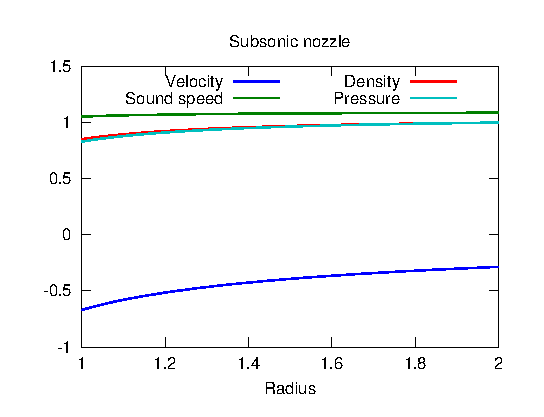
\includegraphics[width=0.80\textwidth]{nozzle_subsonic}
  \vfill
  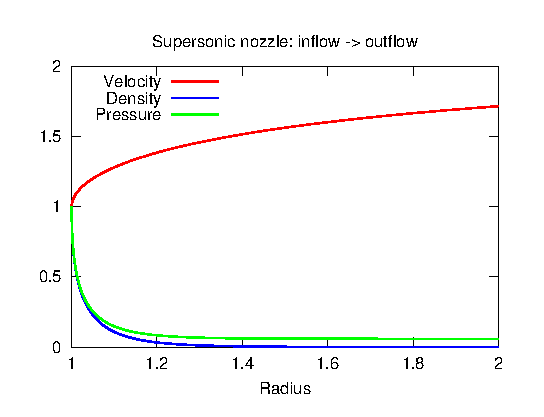
\includegraphics[width=0.80\textwidth]{nozzle_supersonic}
  \caption{
      \label{fig:sample_solns}
      Sample solutions saved by the demo logic in \texttt{nozzle.m}.  The
      subsonic case flows from right-to-left while the supersonic one flows
      from left-to-right.
  }
\end{figure}

\clearpage

%%%%%%%%%%%%%%%%%%%%%%%%%%%%%%%%%%%%%%%%%%%%%%%%%%%%%%%%%%%%%%%%%%%%%%%%%%%%%%%%
\section{Computing quantities of interest for a Cartesian base flow}
%%%%%%%%%%%%%%%%%%%%%%%%%%%%%%%%%%%%%%%%%%%%%%%%%%%%%%%%%%%%%%%%%%%%%%%%%%%%%%%%

\begin{figure}[h]
  \centering
  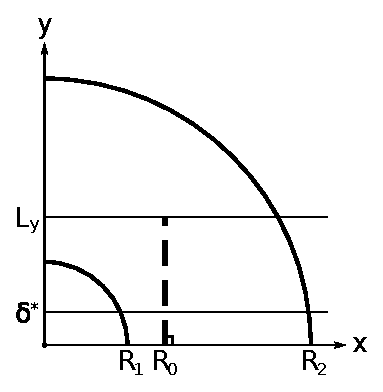
\includegraphics[width=0.38\textwidth]{nozzle_schematic}
  \caption{
      \label{fig:mapping_geometry}
      A Cartesian setting overlaid on the radially symmetric domain
  }
\end{figure}

The favorable pressure gradient base flow profile of height $L_y$ is taken from
a constant $x$ line segment obtained from a radially varying solution.
Referring to Figure~\eqref{fig:mapping_geometry}, the solution
$u\!\left(R\right)$ with accompanying $\rho\!\left(R\right)$,
$p\!\left(R\right)$, and $a\!\left(R\right)$ is valid for
$R\in\left[R_1,R_2\right]$.  For some $\left(x,y\right)$ and corresponding
$R=\sqrt{x^2+y^2}$ one may compute: following:
%
\begin{align}
               \rho \!\left(x, y\right) &= \rho\!\left(R\right)
 &  \partial_x \rho                     &= \frac{x}{R} \rho^\prime\!\left(R\right)
 &  \partial_y \rho                     &= \frac{y}{R} \rho^\prime\!\left(R\right)
\\             u_x  \!\left(x, y\right) &= u   \!\left(R\right) \frac{x}{R}
 &  \partial_x u_x                      &= \frac{1}{R^2}\left[x^2 u^\prime\!\left(R\right) + \frac{y^2}{R} u\!\left(R\right)\right]
 &  \partial_y u_x                      &= \frac{xy}{R^2}\left[u^\prime\!\left(R\right) - \frac{1}{R}u\!\left(R\right)\right]
\\             u_y  \!\left(x, y\right) &= u   \!\left(R\right) \frac{y}{R}
 &  \partial_x u_y                      &= \frac{xy}{R^2}\left[u^\prime\!\left(R\right) - \frac{1}{R}u\!\left(R\right)\right]
 &  \partial_y u_y                      &= \frac{1}{R^2}\left[y^2 u^\prime\!\left(R\right) + \frac{x^2}{R} u\!\left(R\right)\right]
\\             p    \!\left(x, y\right) &= p   \!\left(R\right)
 &  \partial_x p                        &= \frac{x}{R} p^\prime\!\left(R\right)
 &  \partial_y p                        &= \frac{y}{R} p^\prime\!\left(R\right)
\end{align}
% FIXME STARTHERE
\begin{align}
    \rho \!\left(x, y\right) &= \rho\!\left(R\right)
\\  u_\xi\!\left(x, y\right) &= \left|u\!\left(R\right)\right| \frac{x}{R}
\\  u_y  \!\left(x, y\right) &=       u\!\left(R\right)        \frac{y}{R}
\\  p    \!\left(x, y; \Mach\right) &= \frac{\Mach[0]^2}{\Mach^2} \, p\!\left(R\right)
\end{align}
%
Here, $\xi$ denotes the $x$ direction possibly reflected so that streamwise
velocity always has positive sign (i.e. $x$ when $u\geq{}0$, otherwise $-x$).
The $\Mach[0]^2/\Mach^2$ factor permits translating pressure into a
nondimensionalization using some other Mach number $\Mach$ under the assumption
that $p_0 = \rho_0 a_0^2$ holds in the target setting for a possibly different
$a_0$ but $\rho_0$ and $u_0$ remain the same.
%
Differentiation in the streamwise direction $\xi$ and orthogonal $y$ direction
employs, respectively,
\begin{align}
    \frac{\partial}{\partial\xi}
 &= \operatorname{sgn}(u) \frac{\partial}{\partial{}x}
  = \frac{x \operatorname{sgn}(u)}{R} \frac{\partial}{\partial{}R}
&
    \frac{\partial}{\partial{}y}
 &= \frac{y}{R} \frac{\partial}{\partial{}R}
\end{align}
yielding the following:
%
\begin{align}
  \frac{\partial}{\partial\xi} \rho \!\left(x, y\right)
&=
  \frac{x\operatorname{sgn}(u)}{R} \rho^\prime\!\left(R\right)
&
  \frac{\partial}{\partial{}y} \rho \!\left(x, y\right)
&=
  \frac{y                     }{R} \rho^\prime\!\left(R\right)
\\
  \frac{\partial}{\partial\xi} u_\xi\!\left(x, y\right)
&=
  \operatorname{sgn}(u) \left(
      \frac{x^2 u^\prime\!\left(R\right)}{R^2}
    + \frac{y^2 u       \!\left(R\right)}{R^3}
  \right)
&
  \frac{\partial}{\partial{}y} u_\xi\!\left(x, y\right)
&=
  x y \operatorname{sgn}(u) \left(
      \frac{u^\prime\!\left(R\right)}{R^2}
    - \frac{u       \!\left(R\right)}{R^3}
  \right)
\\
  \frac{\partial}{\partial\xi} u_y  \!\left(x, y\right)
&=
  x y \operatorname{sgn}(u) \left(
      \frac{u^\prime\!\left(R\right)}{R^2}
    - \frac{u       \!\left(R\right)}{R^3}
  \right)
&
  \frac{\partial}{\partial{}y} u_y  \!\left(x, y\right)
&=
    \frac{ y^2 u^\prime\!\left(R\right) }{ R^2 }
  + \frac{ x^2 u       \!\left(R\right) }{ R^3 }
\\
  \frac{\partial}{\partial\xi} p    \!\left(x, y; \Mach\right)
&=
  \frac{x\operatorname{sgn}(u)}{R}
  \frac{\Mach[0]^2}{\Mach^2}
  \,
  p^\prime\!\left(R\right)
&
  \frac{\partial}{\partial{}y} p    \!\left(x, y; \Mach\right)
&=
  \frac{y                     }{R}
  \frac{\Mach[0]^2}{\Mach^2}
  \,
  p^\prime\!\left(R\right)
\end{align}
%
A Cartesian flow profile can be extracted from radial solution on the line
segment spanning points $\left(R_0,0\right)$ and $\left(R_0,L_y\right)$ using
these results.  Clearly, selecting
\begin{align}
  R_1 &= R_0
\\
  R_2 &= \sqrt{R_0^2 + L_y^2}
\end{align}
produces the smallest radial domain possessing a solution along this entire
segment.

At some height of interest with such a profile, say an edge distance $\delta$
from the $x$-axis, one may also compute
\begin{align}
  \Mach[e]{}
  &\equiv
  \left. \frac{u_0 u_\xi}{a_0 a} \right|_{\left(R_0,\delta\right)}
  =
  \left.
    \frac{\Mach[0]{} R_0}{R}
    \frac{\left|u\!\left(R\right)\right|}
         {      a\!\left(R\right)       }
  \right|_{R = \sqrt{R_0^2 + \delta^2}}
\end{align}
\begin{align}
  p_{e,\xi}
  &\equiv
  \left.
  \frac{l_0 \delta}{\rho_0 \rho \, u_0^2 u^2}
    \frac{\partial\left(p_0 p\right)}{\partial\left(l_0 \xi\right)}
  \right|_{\left(R_0,\delta\right)}
  =
  \left.
    \frac{\operatorname{sgn}(u) \, \delta}{\Mach[0]^2 \rho u^2}
      \frac{\partial{}p}{\partial{}x}
  \right|_{\left(R_0,\delta\right)}
  =
  \left.
    \frac{\operatorname{sgn}(u) R \, \delta \, p'\!\left(R\right)}
         {\Mach[0]^2 R_0 \, \rho\!\left(R\right) u^2\!\left(R\right)}
  \right|_{R=\sqrt{R_0^2 + \delta^2}}
\end{align}
to interrogate the solution's nature at $\left(R_0, \delta\right)$.  The squared
sound speed at $y=\delta$ and $y=0$ is
\begin{align}
  a^2_e
  &\equiv
  a^2\!\left(\sqrt{R_0^2 + \delta^2}\right)
,
&
  a^2_w
  &\equiv
  a^2\!\left(R_0\right)
.
\end{align}
In the special case of a thermally and calorically perfect gas, these are
nothing but temperatures $T_e$ and $T_w$ because
choices~\eqref{eq:nondimensionalization} imply $a^2 = T$ holds in that
particular context.  A kernel building atop Listing~\ref{lst:octave_nozzle}
that computes these quantities of interest appears in
Listing~\ref{lst:octave_nozzle_qoi}.  By solving to boundary $R_2 = \sqrt{R_0^2
+ \delta^2}$ the kernel both solves the cheapest possible problem and also
causes the ODE integrator to automatically produce full-order results at
$\left(R_0,\delta\right)$ without requiring dense output capabilities.

\lstinputlisting[language=Octave,float=bp,
                 caption={\texttt{nozzle\_qoi.m}: A kernel computing several
                 nozzle quantities of interest\label{lst:octave_nozzle_qoi}}]
                {notebooks/nozzle_qoi.m}

\pagebreak[4]{}

%%%%%%%%%%%%%%%%%%%%%%%%%%%%%%%%%%%%%%%%%%%%%%%%%%%%%%%%%%%%%%%%%%%%%%%%%%%%%%%%
\section{Producing base flows matching given quantities of interest}
%%%%%%%%%%%%%%%%%%%%%%%%%%%%%%%%%%%%%%%%%%%%%%%%%%%%%%%%%%%%%%%%%%%%%%%%%%%%%%%%

A nonlinear optimization problem may be formulated over $\Mach[0]$, $R_0$,
$\rho\!\left(R_1\right)$, and $u\!\left(R_1\right)$ to match some target
$\Mach[e]{}$, $p_{e,\xi}$, and $T_e$ given fixed $\delta$ and $\gamma_0$.
Parameter $p\!\left(R_1\right)$ may be arbitrarily fixed as it does not impact
these particular target quantities.  One possible implementation, written using
the \texttt{nonlim\_resid} method from \texttt{Octave}'s \texttt{optim}
package, is given in Listing~\ref{lst:octave_nozzle_baseflow}.

Several details took considerable effort to refine are therefore worth
noting:\mynobreakpar
\begin{enumerate}
  \item The relative residuals are minimized rather than the absolute residuals
    as otherwise the larger magnitudes of $\Mach[e]{}$ swamp $p_{e,\xi}$
    yielding undesirable results.
  \item A poor initial guess is taken by selecting $R_0 = 10\delta$ and
    $\Mach[0]{}=\Mach[e]{}$.  Choosing $\Mach[0]{}=\Mach[e]{}$ appears to be
    critical for obtaining a range of $a_e^2$ behavior.  This particular value
    stems from investigating what permits~\eqref{eq:stagnation_sound_nondim} to
    produce the necessarily positive $\Mach[0]^2$ when the flow is either
    locally sub- or supersonic.  For subsonic $\Mach[e]{}$ the minimum possible
    $u_1\!\left(R_1\right)$ according
    to~\eqref{eq:cpfradial_nozzle_subsonic_bc} is chosen.  For supersonic
    $\Mach[e]{}$ the mean possible $u_1\!\left(R_1\right)$ according
    to~\eqref{eq:cpfradial_nozzle_supersonic_bc} is selected.
  \item To combat the impact of this poor initial guess, optimization proceeds
   in two phases with the first phase treating only $R_0$ and
   $u\!\left(R_1\right)$ as free parameters.  This first phase is run only
   briefly as otherwise the optimizer sometimes finds a woefully suboptimal
   local minimum.
  \item As shown, $\rho\!\left(R_1\right)$ is taken fixed because because, for
    it to have appreciable impact on the optimization results, the parameter
    often take physically unbecoming values for what should be an order-one
    nondimensional quantity.
\end{enumerate}
All of these choices were required to pass test cases A--F appearing at the end
of Listing~\ref{lst:octave_nozzle_baseflow}.

Not surprisingly, matching $\Mach[e]{}\approx{}1$ taxes this formulation as
implemented here.  Though a realizability constraint is implemented, in practice
it seems not to be encountered by the chosen optimizer with this particular
initialization procedure.  The second \texttt{nonlin\_residmin} invocation
permits many iterations as pre-asymptotic convergence has been quite slow on
one test (not shown).  Generally, fewer than 50 total iterations are required
for convergence to $\sqrt{\epsilon}$-like sum-of-squared mismatch residuals.
After optimization completes, the full base flow profile may be computed by
supplying the results along with $R_2 = \sqrt{R_0^2 + L_y^2}$ to
Listing~\ref{lst:octave_nozzle}.

\lstinputlisting[language=Octave,float=p,
                 caption={\texttt{nozzle\_baseflow.m}: A driver for targeting
                 quantities of interest\label{lst:octave_nozzle_baseflow}},
                 lastline=57]
                {notebooks/nozzle_baseflow.m}

\lstinputlisting[language=Octave,float=p,
                 caption={\texttt{nozzle\_baseflow.m}: Continued},
                 firstline=58,firstnumber=58]
                {notebooks/nozzle_baseflow.m}

\clearpage

%%%%%%%%%%%%%%%%%%%%%%%%%%%%%%%%%%%%%%%%%%%%%%%%%%%%%%%%%%%%%%%%%%%%%%%%%%%%%%%%
\section{Example: Matching laminar CEV heat shield conditions}
%%%%%%%%%%%%%%%%%%%%%%%%%%%%%%%%%%%%%%%%%%%%%%%%%%%%%%%%%%%%%%%%%%%%%%%%%%%%%%%%

A fully laminar Crew Exploration Vehicle (CEV) heat shield problem for peak
heating conditions from an International Space Station return trajectory was
simulated by Paul Bauman of The Center for Predictive Engineering and
Computational Science using the FIN-S hypersonic flow
code\citep{KirkModeling2013}.  Scenario information was gathered along
surface-normal rays on the symmetry plane which are marked with faint lines in
Figure~\ref{fig:cev_symplane}.  The laminar boundary layer character was
quantified as a function of leeward arc length, measured in meters, from the
stagnation region.

\begin{figure}
  \centering
  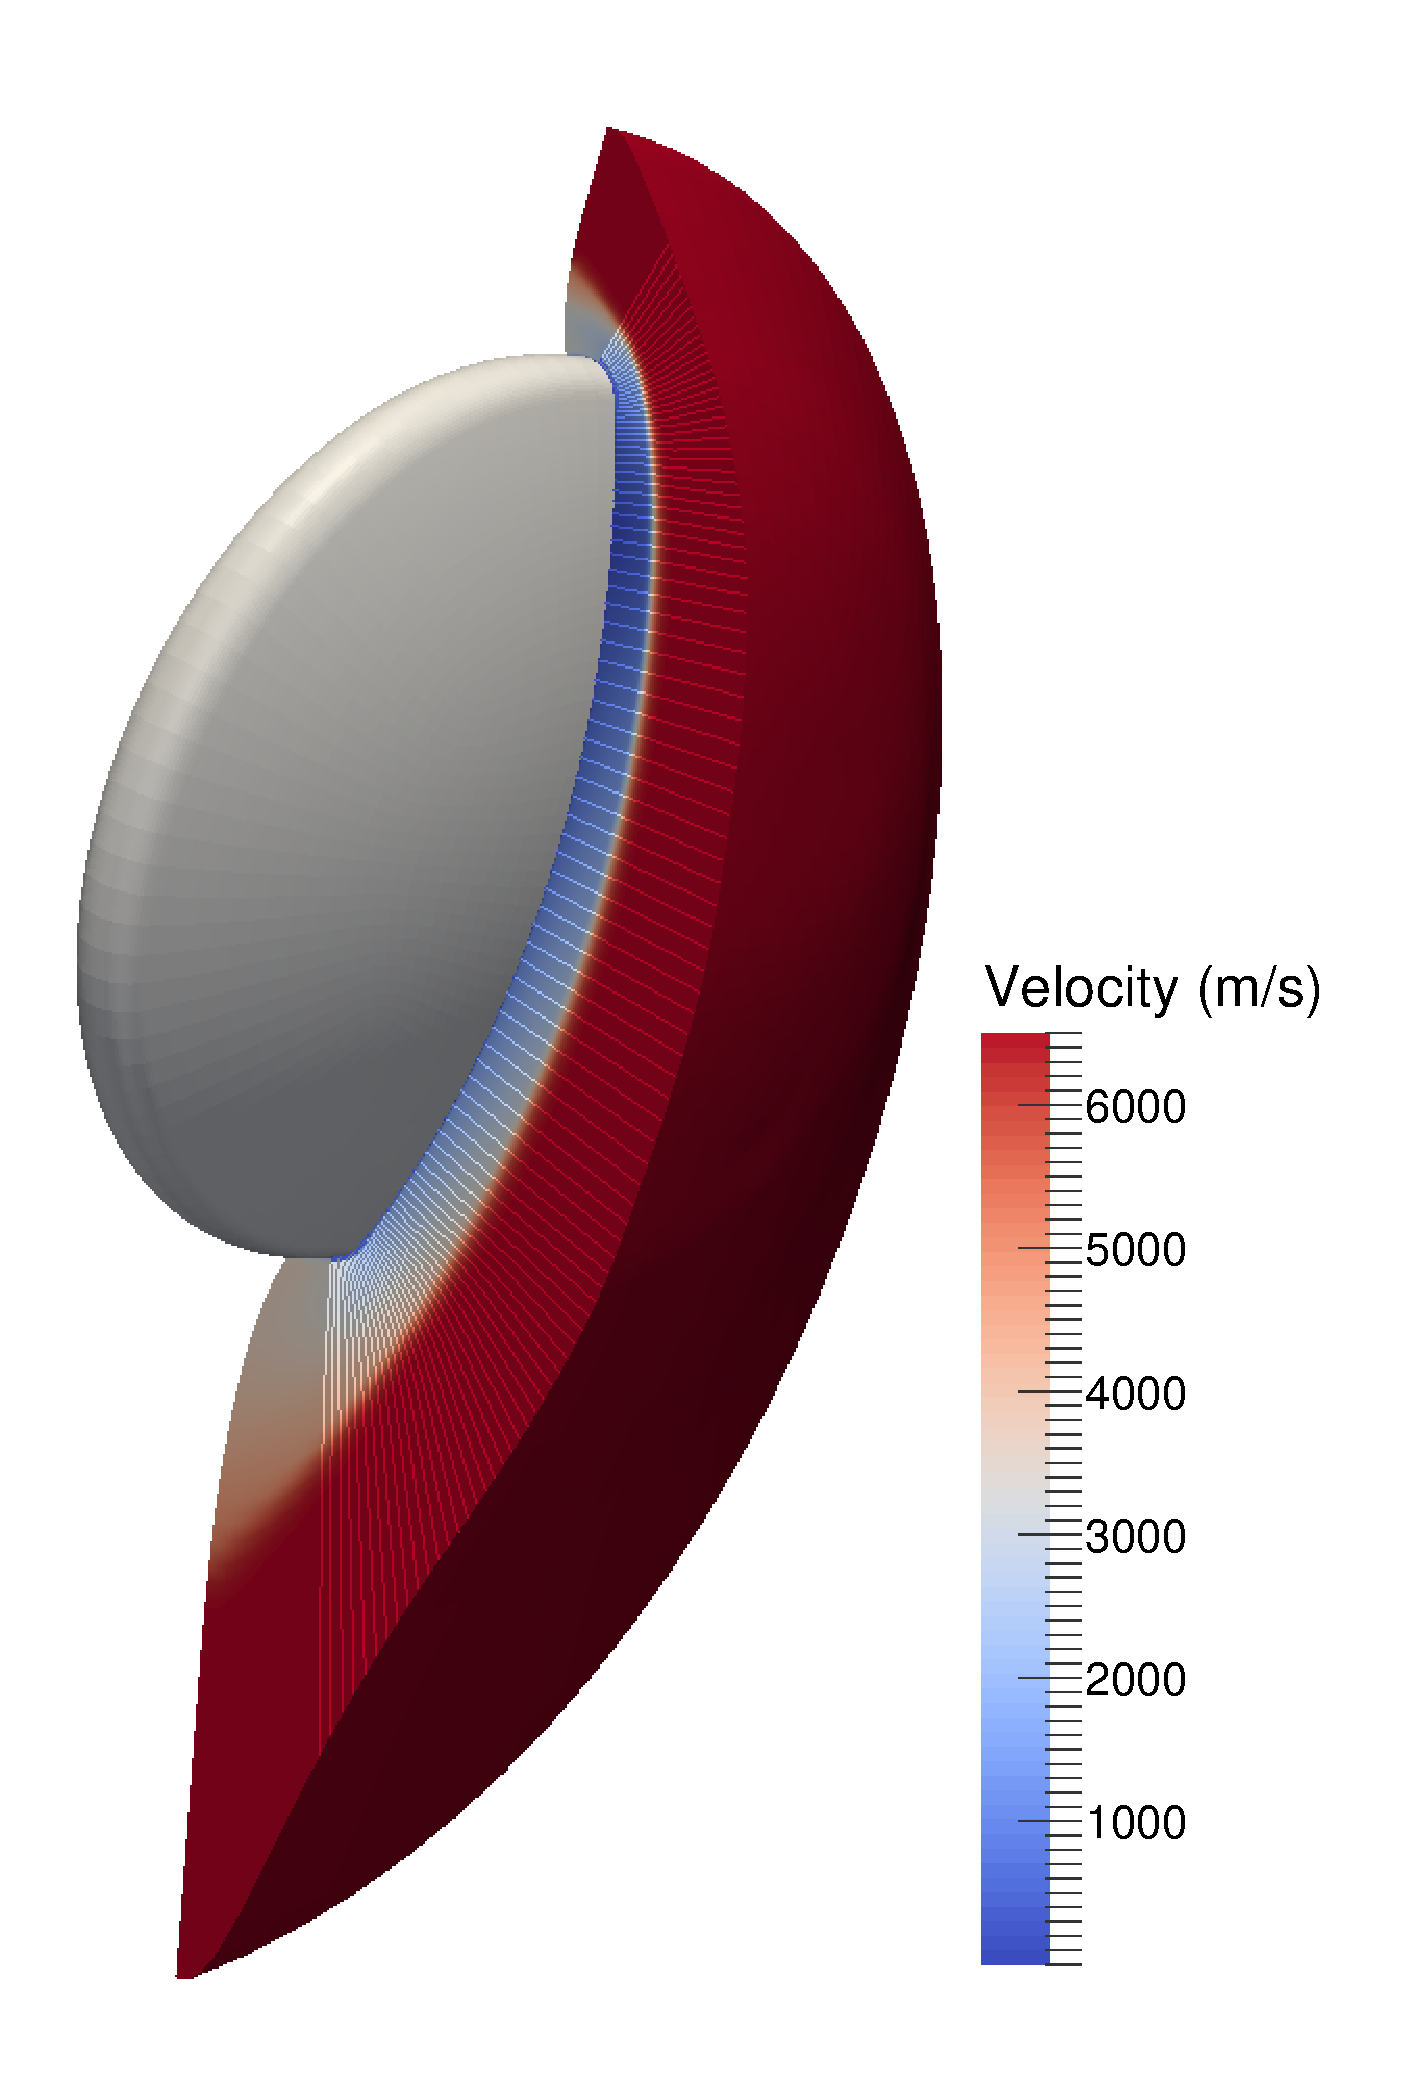
\includegraphics[height=0.55\textheight]{symplanenorm}
  \caption{
    \label{fig:cev_symplane}
    The velocity magnitude on the symmetry plane for the fully laminar
    CEV simulation of interest.
  }
\end{figure}

General boundary layer quantities are plotted in Figure~\ref{fig:cev_summary1}.
Only a few of the plotted quantities are relevant to finding a matching
inviscid base flow.  The ratio of specific heats $\gamma$ and edge Mach number
$\Mach[e]{}$ are taken from the boundary layer edge at distance $\delta$ from
the heat shield surface.  The edge-to-wall temperature $T_e/T_w$ is relevant as
it captures the local speed of sound.  Specifically, for a perfect gas equation
of state nondimensionalized by $a_0^2=\gamma_{0}RT_0$, this ratio defines
nondimensional $a_e^2$ when $a_w^2=T_w=1$ is prescribed as an isothermal wall
condition.  Though present in the CEV simulations and depicted here, heat
shield curvature is neglected.

\begin{figure}[p]
  \centering
  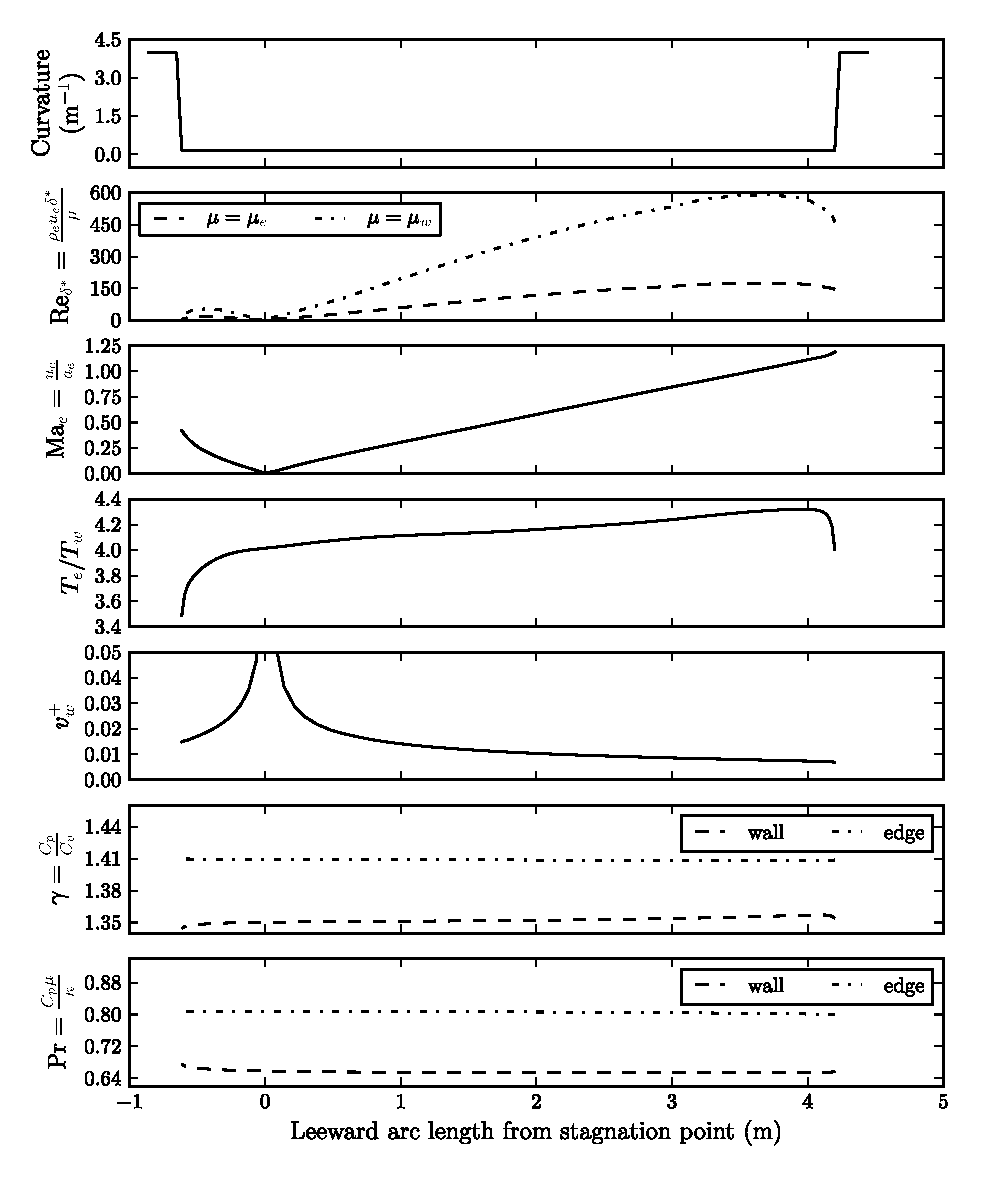
\includegraphics[]{cev_summary1}
  \caption{
    \label{fig:cev_summary1}
    Boundary layer conditions from the fully laminar CEV symmetry plane
  }
\end{figure}

The observed favorable pressure gradient boundary layer nature is quantified in
Figure~\ref{fig:cev_summary_fpg} in a variety of ways.  Of all of these
nondimensional results, $p_{e,\xi}$ is the only quantity with a
directly computable inviscid analog when a target viscous boundary layer
thickness $\delta$ is supplied.  The other nondimensional pressure gradient
parameters, discussed by many authors including
\citet{Sreenivasan1982Laminarescent}, were not adopted for matching purposes as
they require more-complicated flow descriptors like $\delta^\ast$ and $\tau_w$
or the numerically noisy $\frac{\partial\delta}{\partial\xi}$.

\begin{figure}[p]
  \centering
  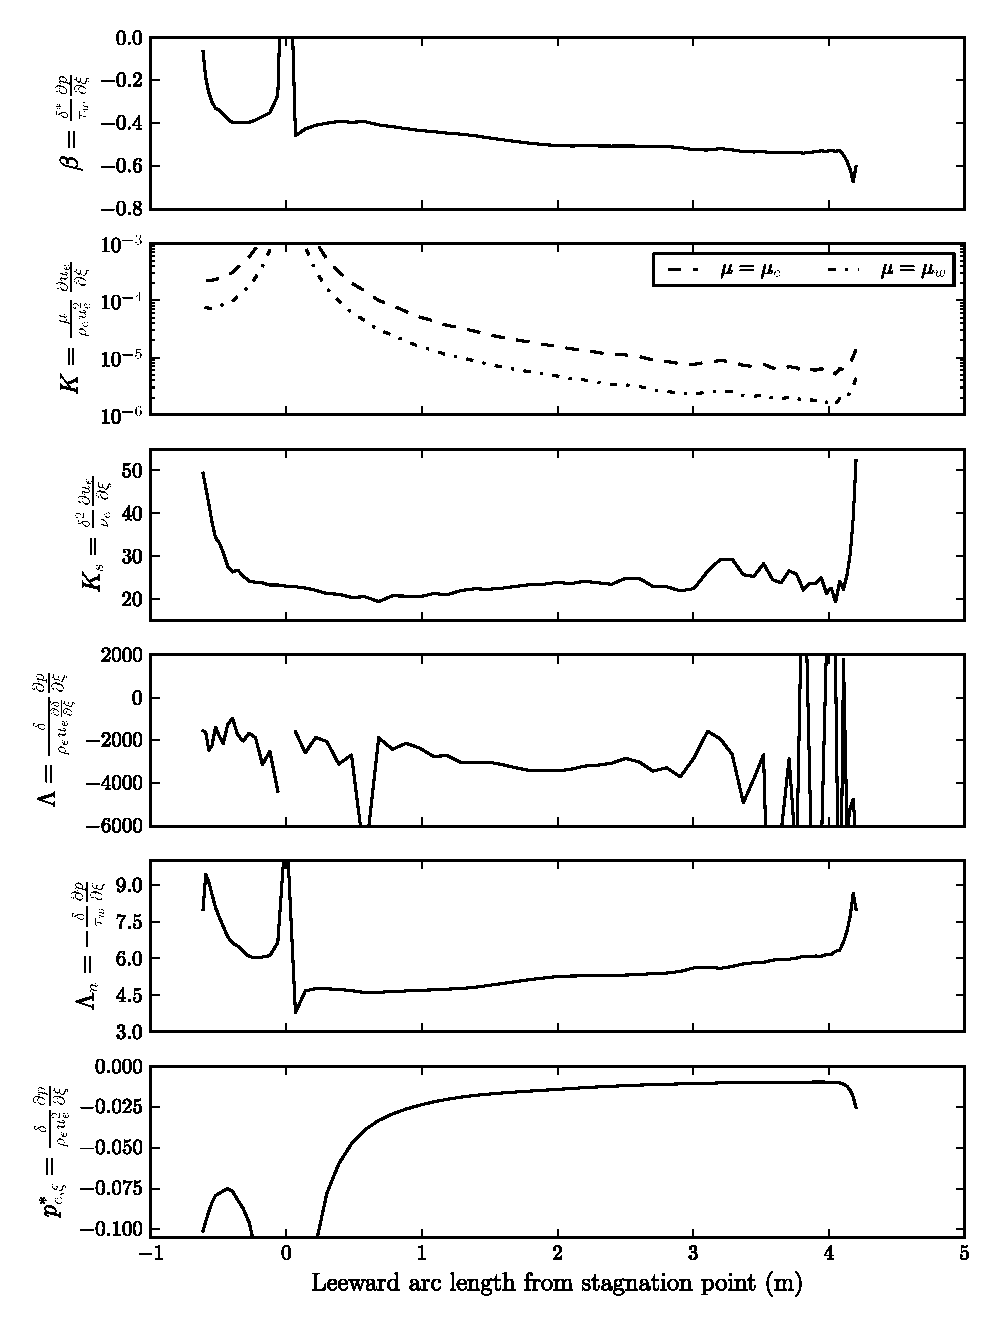
\includegraphics[]{cev_summary_fpg}
  \caption{
    \label{fig:cev_summary_fpg}
    Pressure gradient conditions from the fully laminar CEV symmetry plane.
    Numerical differentiation artifacts are problematic in quantities $\Lambda$
    and $K_s$.
  }
\end{figure}

Conditions $\gamma_e$, $\Mach[e]{}$, $p_{e,\xi}$, and $a^2_e = T_e/T_w$ taken
from the surface-normal rays of Figure~\ref{fig:cev_symplane} were fed into
Listing~\ref{lst:octave_nozzle_baseflow} to produce a family of inviscid base
flow solutions.  The specific values used, rounded to a space-restricted number
of digits, appear below.  As these base flows are intended to be used in a
simulation with roughly nondimensional unit thickness, $\delta=1$ was specified
for all cases.

The resulting solutions are also tabulated below.  Parameters
$\rho\!\left(R_1\right) = 1$ and $p\!\left(R_1\right) = 1$ were fixed with the
remaining $\Mach[0]$, $R_0$, and $u\!\left(R_1\right)$ comprising the problem
space.  Generally, Listing~\ref{lst:octave_nozzle_baseflow} with exactly the
shown initial conditions did a good job of producing solutions with residual
sum of square results less than $\sqrt{\epsilon}$.  However, at arc length
3.586 it is apparent that the solver encountered trouble as it
approached $\Mach[e]{}\approx{}1$.  For reasons unknown, the
\texttt{nonlin\_residmin}-based solver ran afoul of \texttt{NaN}s at arc length
3.287 despite the surrounding cases being well-behaved.  Finally, results from
arc lengths 0.217 to -0.176 are unsatisfying with the hypothesis being that the
strength of the pressure gradient requested as one approaches the stagnation
point being the culprit.

\clearpage

\begin{centering}
\pgfplotstabletypeset[
  col sep=comma
 ,header=true
 ,clear infinite
 ,begin table=\begin{longtable}
 ,end table=\end{longtable}
 ,every head row/.style={after row=\midrule\endhead}
 ,columns={dstag,gamma_e,Ma_edge,p_exi,T_ratio,Ma0,R0,u1,res2}
 ,columns/dstag/.style=  {fixed,fixed zerofill,precision=3,dec sep align,column type/.add={}{|},column name=Arc length}
 ,columns/gamma_e/.style={fixed,fixed zerofill,precision=4,dec sep align,column type/.add={}{},column name=$\gamma_e$}
 ,columns/Ma_edge/.style={fixed,fixed zerofill,precision=6,dec sep align,column type/.add={}{},column name=$\Mach[e]{}$}
 ,columns/p_exi/.style=  {fixed,fixed zerofill,precision=6,dec sep align,column type/.add={}{},column name=$p_{e,\xi}$}
 ,columns/T_ratio/.style={fixed,fixed zerofill,precision=6,dec sep align,column type/.add={}{|},column name=$a^2_e$}
 ,columns/Ma0/.style=    {fixed,fixed zerofill,precision=5,dec sep align,column type/.add={}{},column name=$\Mach[0]{}$}
 ,columns/R0/.style=     {fixed,fixed zerofill,precision=1,dec sep align,column type/.add={}{},column name=$R_0$}
 ,columns/u1/.style=     {fixed,fixed zerofill,precision=5,dec sep align,column type/.add={}{|},column name=$u\!\left(R_1\right)$}
 ,columns/res2/.style=   {sci,  sci   zerofill,precision=0,dec sep align,column type/.add={}{},column name=Residual}
]{notebooks/cev_laminar.out}
\end{centering}

\newcommand*{\doi}[1]{\href{http://dx.doi.org/\detokenize{#1}}{doi: #1}}
\bibliographystyle{plainnat}
\bibliography{references}

\end{document}
